\documentclass[man,11pt,a4paper,floatsintext]{apa7}
% APA 7 professional-manuscript layout in a sans-serif (Helvetica, metrically identical
% to Arial); maths also sans-serif. Converted from the Word original.
\usepackage[T1]{fontenc}
\usepackage[utf8]{inputenc}
\usepackage[scaled]{helvet}
\renewcommand{\familydefault}{\sfdefault}
\usepackage[helvet]{sfmath}
\usepackage{amsmath}
\usepackage{pgfplots}
\pgfplotsset{compat=1.18}
% Figures redrawn from the paper's own functional forms (rho = 0.5, sigma = 1).
% --- Figure 1 ---
\newcommand{\FigOne}{%
\begin{tikzpicture}
\begin{axis}[width=0.78\linewidth, height=6.2cm, axis lines=left, xmin=0, xmax=10.6, ymin=0, ymax=3.75,
  xtick=\empty, ytick=\empty, clip=false,
  xlabel={$N$}, ylabel={$Q$},
  xlabel style={at={(ticklabel* cs:1)}, anchor=north east, yshift=-2pt},
  ylabel style={rotate=-90, at={(ticklabel* cs:1)}, anchor=north east, xshift=-4pt}]
\addplot[very thick, domain=0:10, samples=300] {sqrt(x)};
\node at (axis cs:5.6,3.15) {$Q = AF(K,N)$};
\node[anchor=north east] at (axis cs:0,0) {$0$};
\end{axis}
\end{tikzpicture}}
% --- Figure 2 ---  average output 2/sqrt(N) (dashed) and marginal output 1/sqrt(N) (solid), i.e. rho = 0.5
\newcommand{\FigTwo}{%
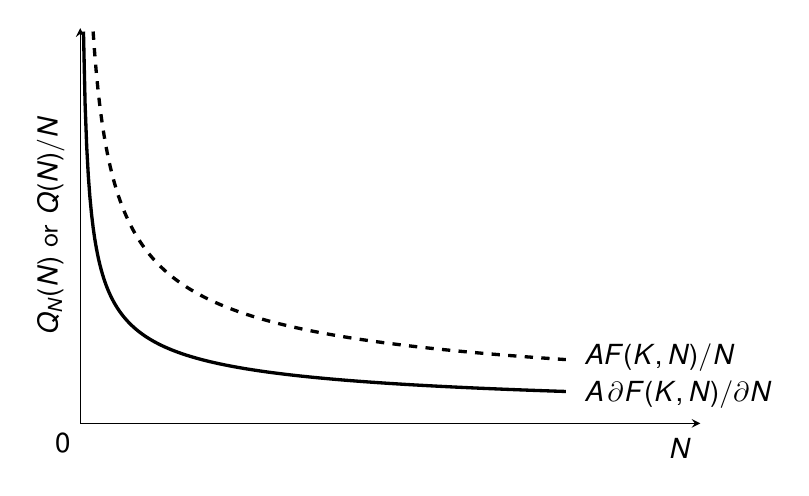
\begin{tikzpicture}
\begin{axis}[width=0.78\linewidth, height=6.6cm, axis lines=left, xmin=0, xmax=10.6, ymin=0, ymax=4.3,
  xtick=\empty, ytick=\empty, clip=false,
  xlabel={$N$}, ylabel={$Q_N(N)$ or $Q(N)/N$},
  xlabel style={at={(ticklabel* cs:1)}, anchor=north east, yshift=-2pt}]
\addplot[very thick, dashed, domain=0.22:8.3, samples=300] {2/sqrt(x)};
\addplot[very thick, domain=0.055:8.3, samples=300] {1/sqrt(x)};
\node[anchor=west] at (axis cs:8.45,0.72) {$AF(K,N)/N$};
\node[anchor=west] at (axis cs:8.45,0.31) {$A\,\partial F(K,N)/\partial N$};
\node[anchor=north east] at (axis cs:0,0) {$0$};
\end{axis}
\end{tikzpicture}}
% --- Figure 3 ---  U(C) = B - 1/C with B = 0.9; zero at C^S = 1/B; the ray from the origin touches the
% curve at C* = 2/B (eq (4): U = CU_C); C^O = 3/B is eq (5) with mu = 1/3 (any mu < 1 puts C^O right of C*)
\newcommand{\FigThree}{%
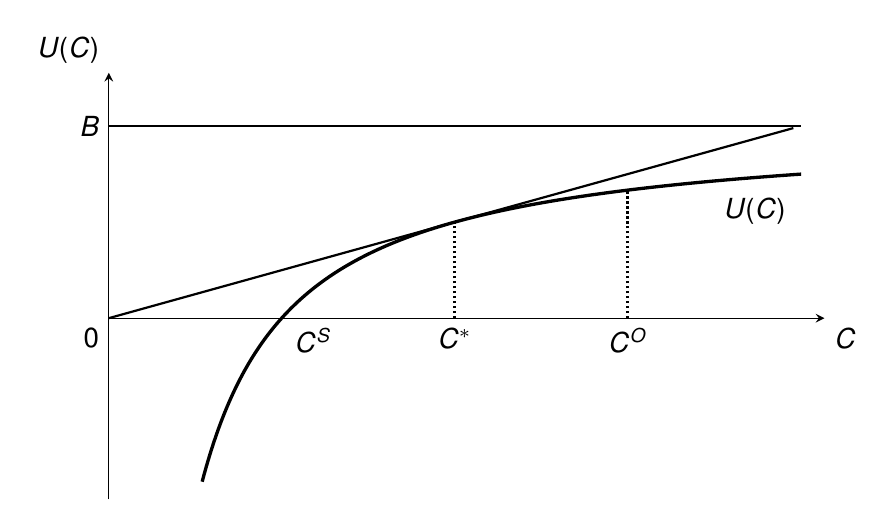
\begin{tikzpicture}
\begin{axis}[width=0.88\linewidth, height=7cm, axis lines=middle, xmin=0, xmax=4.6, ymin=-0.85, ymax=1.15,
  xtick=\empty, ytick=\empty, clip=false,
  xlabel={$C$}, ylabel={$U(C)$},
  xlabel style={anchor=north west}, ylabel style={anchor=south east}]
\addplot[very thick, domain=0.6:4.45, samples=300] {0.9 - 1/x};
\addplot[thick, domain=0:4.45] {0.9};
\addplot[thick, domain=0:4.4] {0.2025*x};
\draw[densely dotted, thick] (axis cs:2.2222,0) -- (axis cs:2.2222,0.45);
\draw[densely dotted, thick] (axis cs:3.3333,0) -- (axis cs:3.3333,0.6);
\node[anchor=north west] at (axis cs:1.13,0) {$C^S$};
\node[anchor=north] at (axis cs:2.2222,0) {$C^*$};
\node[anchor=north] at (axis cs:3.3333,0) {$C^O$};
\node[anchor=east] at (axis cs:0,0.9) {$B$};
\node[anchor=north east] at (axis cs:0,0) {$0$};
\node at (axis cs:4.15,0.5) {$U(C)$};
\end{axis}
\end{tikzpicture}}
\usepackage{url}
\urlstyle{same}

\title{Optimum Population, Global Inequality, and Environmental Constraints: A Utilitarian Perspective}
\shorttitle{OPTIMUM POPULATION AND GLOBAL INEQUALITY}
\authorsnames[1,2]{Partha Dasgupta, SJ Beard}
\authorsaffiliations{{Department of Economics, University of Cambridge},{Centre for the Study of Existential Risk, University of Cambridge}}
\authornote{Acknowledgement: We are most grateful to Aisha Dasgupta for the many discussions we have had on the population-poverty-environment nexus. This project was made possible through the support of grants from the Templeton World Charity Foundation and the Grantham Foundation. The opinions expressed in this publication are those of the authors and do not necessarily reflect the views of these foundations.}
\abstract{In the Utilitarian tradition of Henry Sidgwick, population ethics is to be considered through the expectation of the sum of utilities of all who are ever born. However, this is unsuited for application to the real world because it takes as its subject the choice to be made by an idealized ``objective social planner'' and because it takes as its object a theoretical notion of well-being that is derived from no source and bounded by no constraint. In reality, ethical theories must extend into realms of actual decision-makers, who are subjective agents, and well-being, that is derived from consuming the resources of a finite planet. In this paper, we show how it is possible to amend the utilitarian model by altering the way well-beings are aggregated, to reflect the conditions that are faced by those whose decisions have the greatest impact on demographic change, and to combine it with a more realistic notion of well-being, which takes account of the biosphere's ability to supply humanity with goods and services. To demonstrate the flexibility of this model, we put it to work in investigating a critical question of population ethics that classical utilitarianism cannot contend with, how to explain and respond to differential fertility rates around the world. Our model can be used to study a range of phenomena that may lie behind these differences, including different approaches to property rights over natural resources, different ethical assumptions about the value of children, and the unequal distribution of resources. However, we conclude that there are reasons, not to let these differences stand but to use ethical insights, from our model and elsewhere, to advocate for changes that are likely to be in the long-term interest of humanity.}

\begin{document}
\maketitle
% SJ's choice (not APA): single-spaced footnotes
\makeatletter
\renewcommand\@makefntext[1]{\linespread{1}\selectfont\raggedright\textsuperscript{\@thefnmark}~#1}
\makeatother

While a variety of approaches to population ethics have been proposed, by far the greatest body of academic work has been in the Utilitarian tradition of Henry Sidgwick (1907), who saw the ground of binding reason for choices facing us to be the expectation of the sum of utilities of all who are ever born. We owe a great debt to this tradition and its numerous insights; however, this work is unsuited for application to the world we have come to know, for at least two reasons. The first is that it takes as its subject the choice to be made by an objective social planner, to whom the interests of everyone are equivalent. The second is that it takes as its object an entirely idealized notion of well-being that is neither derived from any particular source nor bounded by any particular constraint. In reality our ethical theories should readily extend into realms in which decision-makers are not objective planners, but subjective agents, and where well-being must be obtained from consuming the resources of a finite planet.

We seek to amend the utilitarian model in two ways. First, we alter the way individual well-beings are aggregated, so they reflect the conditions facing those decision-makers whose choices have the greatest impact on demographic change, namely parents and prospective parents. We contend that the correct choice for parents cannot simply be `derived' from what population ethics might prescribe for an ideal planner, and argue for an alternative theory we call Generation Relative Utilitarianism. Secondly, we show how this theory can accommodate more realistic situations that account for environmental constraints, common pool resources, diverse values, and global inequality.

In Part I we review Sidgwick's Utilitarianism, provide a simplified outline of our alternative theory, and argue that it is better suited to contemporary population ethics. In Part II, we first offer a brief review of what is currently known about the state of the biosphere and what this implies about the flow of goods and services it can supply humanity on a sustainable basis. We then provide an accessible presentation of the application of generation relative utilitarianism to studying earth's carrying capacity and optimal population. In Part III we move onto novel applications of this theory in studying what appears to us to be the crucial next step in applying utilitarian reasoning to global population ethics, by addressing some of the issues that may explain observed differences in fertility rates around the world. We begin with an analysis of how different approaches to the management of commons affect the optimum population size for communities who depend on them. We then briefly consider other possible differentiating factors, relating to cultural differences and economic inequality. We conclude that there are reasons not simply to let these differences stand, but rather to use ethical insights from our model, and elsewhere, to advocate for normative changes that are likely to be in the long-term interest of humanity.

\section{Part I: Parental Utilitarianism and Optimum Household Decision-Making}

\subsection{1 Classical Utilitarian Ethics}

The foundational account of the ethics of population change in analytic philosophy is in the work of the Victorian philosopher Henry Sidgwick. Sidgwick argued for the utilitarian principle that ``the conduct which, under any given circumstances, is objectively right, is that which will produce the greatest amount of happiness on the whole.'' This was not itself a new idea, however, Sidgwick was the first to observe that it raised a question of what we should do when ``an increase in numbers [of people] will be accompanied by a decrease in average happiness or vice versa.'' Sidgwick argued, that under such circumstances:

\begin{quote}
... if we take Utilitarianism to prescribe, as the ultimate end of action, happiness as a whole, and not any individual's happiness, unless considered as an element of the whole, it would follow that, if the additional population enjoy on the whole positive happiness, we ought to weigh the amount of happiness gained by the extra number against the amount lost by the remainder.
\end{quote}

This implies that the basis for evaluation is not gains and losses to people, but gains and losses in total happiness. An ethics grounded on this view sees all happy lives as intrinsically valuable, and hence holds that the better the life is for the person, measured in terms of happiness (or utility), the greater its value. Sidgwick's utilitarianism thus asks us to evaluate alternative states of affairs in terms of the sum of personal utilities, where state of affairs \textit{X} is superior to state of affairs \textit{Y} if total utility in \textit{X} exceeds total utility in \textit{Y}.

This view, which Rawls (1972) called Classical Utilitarianism, has long been known to favour large populations. As we show in section 6.2, if we apply the theory to economic models, it commends a standard of living that is not much higher than that at which their utility is zero (that is, life is neither good nor bad; what Sidgwick called a ``neutral life''). Much work in contemporary population ethics has focused on this implication of the theory, and in particular its purely theoretical implications for population axiology (Broome 2004, Arrhenius et al. 2022). However, these debates have offered little of value to practical considerations.

\subsection{2 Generation Relative Utilitarianism}

In developing alternatives to Classical Utilitarianism, it is worth noting that it involves two related notions: (i) Personal Happiness (or utility) as the valuable property of lives and (ii) summation as the operation for assessing this value.

Sidgwick (1907: 119-150) devotes three chapters to his conception of Personal Happiness, which he terms empirical hedonism; showing that he uses this term far more considerately than is suggested in the frequent criticisms that Classical Utilitarianism views humans to be mere pleasure machines. Nevertheless, we are reluctant to give the impression that the ethical theory we appeal to in this essay relies on Sidgwick's notion of happiness. We therefore modify (i) by using the term ``well-being'', which is generally recognised as capturing the broadest possible conception of personal value.\footnote{Griffin (1986) provides a measured, book-length analysis of this concept in its many guises, but he also develops his preferred interpretation. Briefly, he thinks of personal well-being as a measure of the extent to which one's informed desires are realized. While composing this essay we have kept Griffin's conception in mind, but the mathematical structure of our ethics is not tied to any formulation of well-being.}

The second amendment we make to Sidgwick's theory is a substantial modification of condition (ii). When constructing his version of Utilitarianism, Sidgwick took the position of an objective observer, or planner, to whom ``the good of any one individual is of no more importance \ldots{} than the good of any other'' and which is described as the `Point of View of the Universe.'\footnote{Sidgwick, who was in many ways a humble man, had the grace to write ``the point of view (if I may say so) of the Universe''. However, posterity has preferred this shortened phrase.} We do not believe that this is the appropriate position from which to consider population ethics because, in reality, no such external point of view is available and the decisions that most affect demographic change are the, subjective, choices of parents and prospective parents. This leads us to modify Sidgwick's theory in two key ways. Firstly, we frame all decisions at the household level, where people are choosing the impact of having children upon the well-being of family members, taking account of considerations such as the availability of resources and how these will need to be distributed. Secondly, for reasons we describe below, we will not sum individual well-beings but aggregate them in a way that gives less weight to the well-being of merely potential people than actual people.

We call this modified theory Generation Relative Utilitarianism. Our justification for it is that population ethics is not merely about identifying desirable demographic states of affairs, but also justifying people's reproductive choices. Answers to the latter problem do not follow from resolutions of the former, so we must consider population ethics with regard to both these problems.\footnote{A more complete justification for Generation Relative Utilitarianism is in Dasgupta (2019).}

One modern philosopher who comes close to describing these problems is Scheffler (1982), who pointed to agent-centred concerns, which people can justifiably use as prerogatives, as separate to agent-neutral demands, for deliberating about courses of action open to them (p. 20):

\begin{quote}
... a plausible agent-centred prerogative would allow each agent to assign a certain proportionately greater weight to his own interests than to the interests of other people. It would then allow the agent to promote the non-optimal outcome of his own choosing, provided only that the degree of its inferiority to each of the superior outcomes he could instead promote in no case exceeded, by more than the specified proportion, the degree of sacrifice necessary for him to promote the superior outcome.
\end{quote}

Those prerogatives would apply reciprocally, meaning that in a society of, say, \textit{P} persons the ensuing state of affairs would be the outcome of \textit{P} choices, each guided by separate agent-relative concerns. In population ethics the force of those prerogatives works unidirectionally; so, we make use of an attenuated version of this idea and assume that the decision-maker (here a representative potential parent) evaluates states of affairs on the basis of a weighted sum of personal well-beings, where the weight they place on potential well-beings of children is less than the weight they place on their own well-being. However, we also assume that the decision-maker knows that once this potential person becomes an actual person, i.e. their child is born, they will want to share resources with that child on an equal basis with other family members. There is thus a gap between ex ante and ex post concern for future children that is like nothing we can find in Classical Utilitarianism.\footnote{Scheffler, on the other hand, describes this gap very well, arguing that ``[o]ne cannot value the children one has not yet conceived in the way that one values one's existing children.'' (Scheffler 2018)}

The failure to account for agent-centred prerogatives is not the only thing that has held population ethicists back from making useful contributions to many demographic debates. Of equal importance is their failure to put theories to work in a model where well-being must be derived from a finite stock of natural capital. We turn to this next.

\section{Part II: Optimum Population in the Real World}

\subsection{3 Global Ecological Footprint}

An enormous literature in the environmental sciences records substantial declines in global biodiversity over the past few decades, and consequent reductions in the productivity of ecosystems (Dasgupta 2021). Those declines can be traced to the environmental and reproductive externalities people impose on one another. By ``externalities'' we mean the consequences that our actions have for others but that we are not personally required to account for in our own decision making. In this paper, we frame the idea of optimum population in the context of a finite biosphere and focus on the adverse externalities of our reproductive choices (Dasgupta and Dasgupta 2017). To be sure, the externality we each impose on others is negligible; but when they are summed over many people, the consequences are not.

Today, growth in atmospheric carbon concentration is the canonical expression of adverse externalities, but humanity faces wider and deeper threats to our future from the species extinctions and other reprehensible environmental harm (Dasgupta 2021). Proximate causes of extinctions are destruction and fragmentation of natural habitats and over-exploitation of biological communities; we are converting land into farms and plantations, destroying forests for timber and minerals, applying pesticides and fertilizers to intensify agriculture, introducing foreign species into native habitats, and using the biosphere as a sink for our waste. And these trends are taking place at scales that are orders of magnitude greater than they were even 250 years ago. The Millennium Ecosystem Assessment (2008) reported that 15 of the 24 ecosystems reviewed were either degraded or being exploited at unsustainable rates. Current extinction rates have been estimated to be 10--1,000 times higher than their average over the past several million years (Sodhi, Brook, and Bradshaw, 2009). The World Wildlife Fund (2022) records that between 1970 and 2018 there has been a 69\% decline in the abundance of all monitored wildlife. Studying biogeochemical signatures in sediments and ice of the past 11,000 years, Waters et al. (2016) report that the now-famous figure of the hockey stick characterising the explosive growth of carbon concentration in the atmosphere is also displayed by time series of a broad class of global geochemical signatures. Despite the uncertainties, these findings put the scale of humanity's presence on the Earth system in perspective and explain why our current time has been recognized as the start of a new geological epoch, the Anthropocene.\footnote{Waters et al. (2016) proposed that we regard the mid-20th Century as the time we entered the Anthropocene, as do the Anthropocene Working Group. See Voosen (2016).}

This is consistent with macroeconomic statistics. World population in 1950 was about 2.5 billion, global output of final goods and services was a bit over 8.7 trillion international dollars (Purchasing Power Parity at 2011 prices), and the average person was poor (annual income was around 3,500 international dollars). Since then, the world has prospered beyond recognition. Population has grown to over 7.5 billion and world output of final goods and services is above 110 trillion international dollars (at 2011 prices), meaning that world income per capita is now more than 15,000 international dollars. \footnote{We are deliberately avoiding the more precise estimates of current global GDP and population that are available. Below, we make use of estimates of global ecological footprints that are even cruder than figures for familiar economic and demographic variables and we want to maintain a balance in our exposition. Undue precision of global figures can mislead.} Life expectancy at birth in 1950 was 45, today it is a little over 70. A more than 12-fold increase in global output in a 65-year period helps to explain the stresses to the Earth system we just reviewed.

It also hints at the possibility that humanity's demand for the biosphere's services exceeds sustainable levels. In a review of the state of the biosphere, the World Wildlife Fund (2008) reported that although the global demand for ecological services in the 1960s was less than supply, in the early years of the present century it already exceeded supply by 50 per cent. This figure is based on the idea of ``global ecological footprint,'' the surface area of land and water that would be needed for the Earth system to supply on a sustainable basis the goods and services we consume (food, fibres, wood, water) and to assimilate the waste we produce (materials, gases). The Global Footprint Network (GFN) updates its estimates of the global ecological footprint on a regular basis. A footprint greater than 1 implies that demand for ecological services exceeds their supply, which means there is no way for the world to meet our current requirements sustainably. By GFN's reckoning, it would take 1.7 Earths to sustainably supply sufficient resources to maintain the world's current economy.\footnote{For pioneering work on the idea of ecological footprint, see Rees and Wackernagel (1994) and Rees (2006). See also Kitzes et al. (2008). Wackernagel, who founded the Global Footprint Network, was a lead author of WWF (2008).}

These are \textit{crude} estimates, and we feel nervous using them. Figures for such socio-economic indicators as GDP, population size, and life expectancy are reached by a multitude of national and global institutions, often based on survey data. They are rehearsed regularly, and governments and international agencies use them routinely when advocating and devising policy. We all take note of these figures and trust them. In contrast, we are obliged here to rely on the estimates of a solitary research group (GFN), albeit one with a network of collaborators. Many people will look askance at their estimates. What matters though is not the exact figure but whether we are extracting more resources from the biosphere than it can sustainably supply. On that, there should be little question. That there is an overshoot in global demand for the biosphere's goods and services is entirely consistent with a wide range of evidence on the state of the biosphere (Dasgupta 2021).

Development that relies on extracting more resources than our planet can sustainably supply cannot continue indefinitely. Economic development during the past 65 years has raised the average living standard beyond recognition, even while population has increased by an unprecedented amount; but we have enjoyed that success by leaving a substantially diminished biosphere for future generations. It would appear we are living at once in the best of times and the worst of times. It is hard to be sure what our situation means for the limits of a sustainable world economy. On the one hand, the Global Footprint Network estimates that the last time we had a footprint close to 1 was in 1970, when the global economy was only 15\% of the size it is today. On the other hand, the size of the footprint has shown limited variation over the past 10 years, despite continued global economic growth, suggesting that humanity may be starting to operate more efficiently, in terms of the amount of consumption we can generate from the biosphere.\footnote{Although the nature of that footprint has continued a long-term shift away from localized environmental externalities, such as those produced by over-grazing, and towards global scale destruction, such as climate change.} However, we believe that technological innovations, on their own, will not be sufficient to achieve sustainable outcomes across all of the environmental problems we are creating, and so we assume a roughly linear long-term relationship between the size of the global economy and its impact on the environment. As the estimates from GFN are the only ones on offer for the size of our present overshoot, we make use of them; however, to err on the cautious side we work with a rounded figure of 1.5 for the global ecological footprint. This implies that our planet can sustainably support a global economy of only around 67\% of its present size.

\subsection{4 The Model}

Let us then model what these ecological constraints mean for the optimum population. Below we provide a simplified account of such a model, produced to be accessible for a non-technical audience; however, the full model is presented in Dasgupta (2019). We will turn to novel expansions and applications of this model in Part III.

We will think of the biosphere as the stock of global capital assets of size \textit{K}. Labour, working on the biosphere, produces outputs for our consumption. It may seem as though this neglects the role of produced capital (roads, buildings, machines etc); but to avoid too much complexity we will simply imagine that substitution possibilities between produced capital and the biosphere are extremely limited, so that the stock of produced capital is, literally, built into \textit{K}.\footnote{Throughout this paper, we assume that all consumption goods are produced by the conjunction of labour and a combination of produced capital and the biosphere.}

For simplicity, our model will be timeless, in that the output is consumed entirely without the possibility of saving for the future. This enables us to investigate the optimum population and living standard humanity should aim for, without worrying about how we get there. The optimization exercise is conducted in two stages. In the first stage the world is populated only by adults, who are assumed to be identical in every way. This means that any one of them can serve as a proxy decision-maker whose choices will be reflected across the entire population. This decision-maker chooses how many children to have, and hence the size of the next generation. These children are identical to the adults in their propensity to consume, but do not offer any labour (children don't work in this model). In the second stage the adult population applies its labour to the biosphere to produce output. That output is consumed equally by the entire population. Even though it is timeless, the model mimics a dynamic model in a stationary mode in which people live for two periods, consuming in both but producing only when they are adults.\footnote{A formal demonstration of this is in Dasgupta (2019).}

\subsubsection{4.1 Production and Consumption}

Let us set the number of people in the global population at \textit{N}\textsubscript{0}. All these people are identical in every respect, including our representative decision-maker whose choices thus serve as a proxy for the choices of all \textit{N}\textsubscript{0} people. And, as we are studying optimum global population, we assume that all other externalities have been eliminated, so that the choices of our decision-maker control the use of the biosphere. As the model is timeless, each individual's life cycle is embedded in it. If \textit{C} is someone's consumption level - we may call it their ``living standard'' - their personal well-being is \textit{U}(\textit{C}). The problem facing our decision-maker is to determine the number of people to add, by having children. We assume that the world is not already overly populated, which means \textit{K} is large relative to \textit{N}\textsubscript{0}. It also means that if they were not to have children, each person would enjoy a high standard of living. If they do have children, they will share whatever output they produce among all on an equal basis. So, adding to their numbers will cost the adults but, because they are Generation Relative Utilitarians, they will still have children if they judge that these children will benefit enough to outweigh these costs.

Let \textit{Q} be output of consumption goods. This will be determined by a function of \textit{N} (the population size, here equal to N\textsubscript{0}) and \textit{K} (the stock of global capital assets representing the biosphere) that is homogeneous of degree 1 (i.e., doubling both \textit{N} and \textit{K} doubles output, while increasing either one alone raises output at a diminishing rate), call this \textit{F(K,N),} together with the ``total factor productivity'' (\textit{A}), interpreted as an aggregate measure of the society's knowledge base and its institutions. This can be written as follows:

\begin{equation}
Q = AF(K,N), \qquad A > 0
\tag{1}
\end{equation}

\noindent \textit{A} is a parameter in the model, not a variable, and, because the model is timeless, we take \textit{K} to be a parameter as well. Assuming that if either \textit{K} or \textit{N} is 0 then F will also be zero, this equation yields the relationship between total production and population size illustrated in Figure 1.

\begin{figure}[htbp]
\caption{Population Size and Total Output}
\centering
\FigOne
\end{figure}

Notice also that average output per worker (that is, \textit{AF}(\textit{K},\textit{N})/\textit{N}) is a declining function of the number of workers. It follows that the marginal output of additional workers ($\partial$AF(K,N)/$\partial$N) is also declining with N, and is constantly below this average. This is shown in Figure 2.

\begin{figure}[htbp]
\caption{Population Size and Average and Marginal Outputs}
\centering
\FigTwo
\end{figure}

To determine the quantity of well-being (\textit{U}) from this output (\textit{Q}) we need to combine this equation with a model for individual well-beings. We assume that well-being increases with consumption (\textit{C}) but at a diminishing rate. The marginal well-being of consumption (d\textit{U}(\textit{C})/d\textit{C}) can be written as \textit{U}\textsubscript{\textit{C}}, and the change in marginal well-being of consumption (d\textsuperscript{2}\textit{U}/d\textit{C}\textsuperscript{2}) as \textit{U}\textsubscript{\textit{CC}}. Thus, \textit{U}\textsubscript{\textit{C}} is always greater than 0 and \textit{U}\textsubscript{\textit{CC}} less than 0. A positive level of well-being (\textit{U} \textgreater{} 0) indicates that life is good for the person living it, negative well-being (\textit{U} \textless{} 0) that it is not good. \textit{U} will be positive for larger values of \textit{C} but negative at smaller values of \textit{C}, so there is a unique level of consumption (i.e., value of \textit{C}) at which \textit{U} is zero. Meade (1955) called the standard of living at which \textit{U} = 0 ``welfare subsistence''; however, in keeping with our axiology we will refer to it as ``well-being subsistence'' and write it as \textit{C}\textsuperscript{\textit{S}} as illustrated in figure 3 below.

Earth's carrying capacity is the human population size that the biosphere can support when everyone is at well-being subsistence. Let us label this 2\textit{N}\textsuperscript{\textit{S}} (it will become evident why we introduce the factor 2 when we come to calculate Earth's carrying capacity in section 6.2).

\subsection{5 Applying Generation Relative Utilitarianism}

The choices facing our decision-maker involve two stages. In the first stage they choose how many children to have, and hence the number of people to be created (\textit{N}\textsubscript{1}). We assume that each of those \textit{N}\textsubscript{1} people will have the same \textit{U}-function as the \textit{N}\textsubscript{0} adults. In making that choice, our decision-maker knows that once born, the additional people will join the existing population as consumers (but not as producers) and enjoy the same status as themselves. Production (Q) and consumption take place in the second stage. Given this, our decision-maker knows that while the production of goods will be determined by the function \textit{AF}(\textit{K},\textit{N}\textsubscript{0}), where \textit{N}\textsubscript{0} is the number of productive adults alive at this time, but consumption will be shared equally among a larger population of size \textit{N}\textsubscript{0}+\textit{N}\textsubscript{1}, where \textit{N}\textsubscript{1} is the number of children they and their fellow parents decide to have. Each person's living standard (\textit{C}) will thus be \textit{AF}(\textit{K},\textit{N}\textsubscript{0})/(\textit{N}\textsubscript{0}+\textit{N}\textsubscript{1}). This is shown in Figure 3 below.

How should our decision-maker evaluate this outcome? According to classical utilitarianism they simply work out the total quantity of well-being that will be produced. However, this does not reflect the values that parents actually have. While our decision-maker knows in advance that they will love their children and share resources equally with them once they are born, that doesn't mean they value their prospective children's well-being now as much as their own. The weight awarded by our decision-maker to the own well-being of the existing population is 1; however, the weight she awards to the well-being of potential people is $\mu$, where 0 \textless{} $\mu$ \textless{} 1. We will discuss the size and justification for this weighting in section 6.2 and again in section 9.

It will be noticed that Generation Relative Utilitarianism invokes only a weak form of agent-centred prerogatives, where these are relative to our position in time but not in space. The theory gives less weight to the well-being of prospective future people, it doesn't sanction applying a lower weight on others' well-being now. Nevertheless, depending on the relative weights deployed by our decision-maker, the gap between ex ante and ex post reasoning can have huge implications for optimum population size.

\subsection{6 Optimum Population and Consumption}

Under Generation Relative Utilitarianism, we require a new term to describe decision-makers' evaluations of all well-being, whether actual or prospective, let us call this \textit{V}. Because her perspective plays a role in that conception, we will call \textit{V} her \textit{social valuation function}. Given that \textit{C} = \textit{AF}(\textit{K},\textit{N}\textsubscript{0})/(\textit{N}\textsubscript{0}+\textit{N}\textsubscript{1}):

\begin{equation}
V = N_0U(AF(K,N_0)/(N_0+N_1)) + \mu N_1U(AF(K,N_0)/(N_0+N_1))
\tag{2}
\end{equation}

\noindent That is, V consists of the total well-being from \textit{N}\textsubscript{0}'s consumption of their fair share of global outputs together with the total well-being from \textit{N}\textsubscript{1}'s consumption of their fair share, multiplied by our decision-maker's weighting $\mu$.

\subsubsection{6.1 Basics}

The problem before our decision-maker is to choose \textit{N}\textsubscript{1} so as to maximize \textit{V}. At this optimum, neither a small hypothetical increase in population, nor a small hypothetical decrease, would alter our decision-maker's evaluation of states of affairs. Suppose they contemplate a marginal increase in numbers (i.e., they contemplate having an additional child). Any additional person, who is only a potential person in the calculation, would be entitled to an equal share of global outputs (\textit{Q)}. They would add their personal well-being to the total, given the current level of consumption, that is \textit{U}(\textit{C}), but there would also be a decrease in well-being because all other people (actual or potential) would have their own shares of \textit{Q }slightly reduced. Summed over everyone, that loss is \textit{CU}\textsubscript{\textit{C}}: the marginal well-being of consumption, \textit{U}\textsubscript{\textit{C}}, multiplied by the standard of living, \textit{C}. Generation Relative Utilitarianism requires that, as there are N\textsubscript{0} actual persons and N\textsubscript{1} potential persons, our decision-maker should count this loss (\textit{N}\textsubscript{0}+$\mu$\textit{N}\textsubscript{1})/$\mu$(\textit{N}\textsubscript{0}+\textit{N}\textsubscript{1}) times as heavily as the additional person's own well-being, which carries a weight of only $\mu$ because they are a potential person. If they were to consider having fewer children instead, then their deliberations would be analogous.

At the optimum, the potential gain and the potential loss in \textit{V}, from either an increase or a decrease in population size, must be equal. So, the optimum size for \textit{N}\textsubscript{1} is that which satisfies:

\begin{equation}
U(C) = [(N_0+\mu N_1)/\mu(N_0+N_1)]CU_C \quad > 0
\tag{3}
\end{equation}

Since Classical Utilitarianism effectively sets $\mu$ = 1, equation (3) would reduce to the condition:

\begin{equation}
U(C) = CU_C
\tag{4}
\end{equation}

\noindent Call the standard of living in equation (4) \textit{C}*. Figure 3, below, shows that at \textit{C}* average well-being per unit of consumption equals marginal well-being.

In contrast, according to Generation Relative Utilitarianism $\mu$ should be less than 1. In that case (\textit{N}\textsubscript{0}+$\mu$\textit{N}\textsubscript{1}) would be greater than $\mu$(\textit{N}\textsubscript{0}+\textit{N}\textsubscript{1}). Equation (3) now says that at the optimum, \textit{U}(\textit{C}) \textgreater{} \textit{CU}\textsubscript{\textit{C}}. Notice also that the smaller is $\mu$, the greater is the difference between \textit{U}(\textit{C}) and \textit{CU}\textsubscript{\textit{C}}, which in turn implies that the optimum standard of living is higher. This is demonstrated in Figure 3 below.

\subsubsection{6.2 Reproductive Replacement}

Now, imagine that the optimum policy for the existing population is to replicate itself. That's when \textit{N}\textsubscript{0} just \textit{happens} to be a figure for which the optimum size for \textit{N}\textsubscript{1} equals the actual size of \textit{N}\textsubscript{0}. The reason we are interested in this extreme scenario, is that it mimics an economy moving through time in a \textit{stationary} state, in this case one where people live for two periods and produce 1 child per person at the beginning of their second period.

So, in our timeless economy, we set \textit{N = N}\textsubscript{0} = \textit{N}\textsubscript{1}. Total population is then 2\textit{N}, and the optimality condition (eq. (3)) becomes:

\begin{equation}
U(C) = [(1+\mu)/2\mu]CU_C
\tag{5}
\end{equation}

\noindent Let the solution of equation (5) be denoted as \textit{C}\textsuperscript{\textit{O}}. That is to say, \textit{C}\textsuperscript{\textit{O}} is the optimum living standard under Generation Relative Utilitarianism.

Under Classical Utilitarianism's $\mu$ = 1, equation (5) again reduces to the condition

\begin{equation}
U(C) = CU_C
\tag{6}
\end{equation}

\noindent We have dubbed the solution of equation (6) as \textit{C}*. A comparison of equations (5) and (6) tells us immediately that \textit{C}\textsuperscript{\textit{O}} \textgreater{} \textit{C}*, i.e., that the standard of living will be higher in this steady state world if our decision-maker follows generation relative utilitarianism than if they follow classical utilitarianism.

We can go further with these equations if we adopt simple forms of the production function \textit{AF}(\textit{K,N}) and the well-being function \textit{U}(\textit{C}). Their simplest expressions are the following two power functions:

The production function is:

\begin{equation}
AF(K,N) = AK^{(1-\rho)}N^{\rho}, \qquad A > 0, \quad 0 \le \rho < 1
\tag{7}
\end{equation}

\noindent This equation is widely used by economists to reflect production possibilities. The parameter $\rho$ reflects the productivity of labour. Output is an unbounded function of population numbers, but Nature imposes a restraint on the rate at which output can expand with population. The latter is reflected in the condition $\rho$ \textless{} 1. (1-$\rho$) is the productivity of \textit{K}. Ideal national income accounting would interpret $\rho$ to be the share of total output attributable to labour. There is an enormous empirical literature offering estimates of $\rho$. They tend to lie in the range 0.6-0.7. Because we are including the biosphere in the accounts, $\rho$ should be taken to be smaller. In numerical exercises we will assume, solely for computational ease, that $\rho$ = 0.5.

The well-being function is:

\begin{equation}
U(C) = B-C^{-\sigma}, \qquad B > 0, \quad \sigma > 0
\tag{8}
\end{equation}

\noindent This defines \textit{U}(\textit{C}) by two parameters, \textit{B} and $\sigma$, both positive numbers. In this function, marginal well-being declines quickly enough that there is a highest possible level of well-being that anyone could achieve, regardless of their consumption. Ramsey (1928) refers to this as `Bliss' and we write it as \textit{B}. 1+$\sigma$ is called the ``elasticity of marginal well-being with respect to consumption'' and is the absolute value of the percentage rate at which marginal well-being changes with each percentage rate of increase in consumption (i.e., 1+$\sigma$ = -dlog(\textit{U}\textsubscript{\textit{C}})/dlog\textit{C}). This elasticity exceeds 1 in the \textit{U}-function of equation (8). It is easy to show that, if \textit{U}(\textit{C}) satisfies equation (8), then \textit{C}\textsuperscript{\textit{S}} = \textit{B}\textsuperscript{-1/$\sigma$}.

We can now work with these functions to study equation (5). Under Sidgwick's Utilitarianism, where $\mu$ = 1, applying equation (8) to equation (5) yields:

\begin{equation}
C^*/C^S = [1+\sigma]^{1/\sigma} \quad < e \approx 2.7\ldots
\tag{9}
\end{equation}

\noindent This equation tells us that the optimum standard of living under classical utilitarianism (C*) can be no greater than \textasciitilde{}2.7 times well-being subsistence (\textit{C}\textsuperscript{\textit{S}}) (Dasgupta, 1969).

In contrast, the optimum living standard can be far higher under Generation Relative Utilitarianism. The smaller the relative weight our decision-maker gives to prospective over actual well-being (\textit{$\mu$}), the higher this standard (\textit{C}\textsuperscript{\textit{O}}) will be. To confirm, recall that we defined Earth's carrying capacity as the size of the global population that the biosphere could sustain at a standard of living equal to well-being subsistence. We denoted the size of that population by 2\textit{N}\textsuperscript{\textit{S}}. Thus, Earth's carrying capacity is given by the following equation:

\begin{equation}
AK^{(1-\rho)}(N^S)^{\rho}/2N^S = C^S
\tag{10}
\end{equation}

\noindent Applying the well-being and productivity functions (7) and (8) to equation (5) to determine the optimum living standard, and comparing this with equation (10) yields the result that:

\begin{equation}
C^O/C^S = (N^S/N^O)^{(1-\rho)} = [1+(1+\mu)\sigma/2\mu]^{1/\sigma}
\tag{11}
\end{equation}

\noindent As expected, we can see that \textit{C}* in equation (9) will be smaller than \textit{C}\textsuperscript{\textit{O}} in equation (11), and the smaller is $\mu$ the larger this difference will be (since $\mu$ is less than 1, dividing by $\mu$ makes this term larger). Figure 3 illustrates this. \textit{C}* is the consumption level at which average well-being per unit of consumption equals marginal well-being, which is where a straight line from the origin just touches the well-being curve. \textit{C}\textsuperscript{\textit{O}} always lies to the right of \textit{C}*, and the smaller is $\mu$, the further to the right it lies.

\begin{figure}[htbp]
\caption{Personal Well-Being and the Standard of Living}
\centering
\FigThree
\end{figure}

To obtain a quantitative assessment of the optimum population under Generation Relative Utilitarianism, we need numerical values of $\rho$, $\sigma$ and $\mu$. As described above, we assume $\rho$ = 0.5. Many economists have estimated $\sigma$ from consumption behaviour under risk. For ease of computation we settle for a value of $\sigma$ = 1, which is at the upper end of the range that has been found in empirical studies. Casual empiricism on health and education expenditures in time and money on children in the West (where children most nearly approximate our model as pure consumers and not producers) suggest that $\mu$ is considerably less than 1. People seem to place far greater weight on the well-being of their children than on the potential well-being of children who might have been born but weren't because couples chose not to have further children. No doubt household behaviour isn't the exclusive source of ethical understanding, but it would be wrong to ignore people's intentions altogether in reaching ethical directives. For illustration, let us assume $\mu$ = 0.05. This is to take a lunge in the dark, but we are using the figure only for illustrative purposes.

Applying these figures to equation (11) yields 2\textit{N}\textsuperscript{\textit{S}}/2\textit{N}\textsuperscript{\textit{O}} $\approx$ 132, meaning that the biosphere's carrying capacity for humans is (approximately) 132 times the optimum population, according to generation relative utilitarianism. This is a far cry from the ratio for Total Utilitarianism, which (setting $\mu$ = 1 in equation (11)) is 4.

Obtaining actual figures for Earth's carrying capacity and optimum population is also possible, although to do this we need to estimate the biosphere's productivity and its regenerative possibilities. In other work Dasgupta (2019) used an estimate for total size of global production (\textit{AK}\textsuperscript{(1-$\rho$)}(\textit{N})\textsuperscript{$\rho$}) of around 110 trillion international dollars. With $\rho$ = 0.5 and roughly 3.75 billion producers, this implies a value of about 1.8 billion for \textit{AK}\textsuperscript{(1-$\rho$)}, which measures the combined productive capacity of the biosphere and all other capital assets. As we assume a linear relationship between the size of our economy and its impact on the biosphere and that the global economy currently has a footprint of 1.5 earths, it follows that the sustainable value of this term is about 1.2 billion. We can now calculate Earth's carrying capacity (2\textit{N}\textsuperscript{\textit{S}}) using equation (10) and its optimal population under Generation Relative Utilitarianism (2\textit{N}\textsuperscript{\textit{O}}) using equation (11). Given that we assume $\rho$ = 0.5 and \textit{C}\textsuperscript{\textit{S}} = 1,500 international dollars, Earth's carrying capacity (2\textit{N}\textsuperscript{\textit{S}}) will be 320 billion and the optimal global population (2\textit{N}\textsuperscript{\textit{O}}) will be 2.4 billion, while Classical Utilitarianism would recommend a far higher global population of 80 billion!\footnote{See also Dasgupta, Dasgupta, and Barrett (2023) for another method for estimating these values.}

\section{Part III: Reconciling Generation Relative Utilitarianism With Differential Fertility and Global Inequality}

\subsection{7 Decentralizing the Optimum}

In formulating the problem of optimum population, we assumed that our decision-maker's choices enforce the \textit{full optimum}, i.e. that the only constraints they face are those on aggregate production possibilities (eq. (1)). Because people in our model are undifferentiated, having identical \textit{U}-functions, the decision-maker does not discriminate among households in any way.

From equation (11) we can note that both \textit{C}\textsuperscript{\textit{O}}\textit{/C}\textsuperscript{\textit{S}} and \textit{N}\textsuperscript{\textit{O}}\textit{/N}\textsuperscript{\textit{S}} are independent of \textit{AK}\textsuperscript{(1-$\rho$)}, the combined productive capacity of the biosphere and all other capital assets.\footnote{Although they are still subject to the assumption of constant returns to scale of the production function (\textit{eq (7)}).} This is a striking feature of the Utilitarian calculus, be it the Classical or the Generation Relative version; well-being subsistence is based solely on the well-being function and does not depend on production possibilities. \textit{AK}\textsuperscript{(1-$\rho$)}, in contrast, only expresses the economy's production possibilities, not what we should do with them. So, equation (11) says that the living standard at the full optimum is independent of \textit{AK}\textsuperscript{(1-$\rho$)}. On the other hand, equation (10) says that Earth's carrying capacity, 2\textit{N}\textsuperscript{\textit{S}}, depends both on \textit{C}\textsuperscript{\textit{S}} and the economy's production possibilities. For any estimated value of \textit{C}\textsuperscript{\textit{S}}, the larger is \textit{AK}\textsuperscript{(1-$\rho$)} the larger Earth's carrying capacity will be, and the optimum population will be larger by the same proportion.

What if we weaken the assumption that people are undifferentiated, so that we continue assuming that all people follow the same well-being function and level of well-being subsistence, C\textsuperscript{S}, but now have them starting with different incomes? On our model, decision-makers from higher income households should choose to have more children than those from lower income households; with all households aiming to end up at the same optimum consumption level by sharing their different greater or fewer resources among more or less children.

It should be immediately apparent that this finding does not cohere with the observations of economic demography, since not only do different people choose to have different numbers of children but there is a general trend for poorer households to have more children than richer ones, both within and between countries (Schultz 2006). Of course, this trend hides many important counterexamples, for instance among some rapidly developing countries with very low fertility and some wealthy families who appear to use their wealth to have more children than their poorer peers.\footnote{Furthermore, it should be noted that many of the countries with the very lowest fertility rates are middle-income countries, such as Brazil (1.65), Romania (1.58), Iran (1.54), Thailand (1.42), and Moldova (1.24).} However, the general trend remains a problem for our model because, while it is easy to say that people are, for a variety of reasons, simply making the wrong choices; if people's choices are the inverse to what our model indicates they should be then this suggests that either we have failed to capture some ethically salient features of their situation or they are simply not engaging in ethical reasoning when deciding whether to have children.

Among economists, a now-traditional explanation for this trend is based on the (market) value of time (Becker, 1960; Becker, Murphy, and Tamura, 1990). Wealthier households are wealthier because, the argument goes, their wages are higher, and their wages are higher because they have acquired more human capital (e.g., education) than less wealthy households. So, the value of time is higher for wealthier households. If one acknowledges that bearing and rearing children is very time consuming, this may explain the trend. However, this explanation is restricted to market economies. The Beckerian framework does not work well in poor countries, because rural women there are required to do a huge amount of work both in and out of the home.

In the next two sections we will therefore consider two other possible factors that may help explain this apparent discrepancy between what our model says about the optimum behaviour for decision-makers and what people are actually choosing to do. For a review of many other social factors that affect fertility decisions in poor countries, see Dasgupta (1993).

\subsection{8 The Biosphere as a Differentiated Commodity}

Adverse externalities from our use of the biosphere arise, in great measure, because Nature is mobile: birds and insects fly, water flows, the wind blows, and the oceans circulate. That makes it hard to establish property rights to key components of the biosphere. By property rights we don't only mean private rights, but also include communitarian and public rights; since much of the biosphere is an ``open-access resource,'' meaning that it is free to all to use as they wish. Hardin (1968) famously spoke of the fate of non-managed common property resources as ``the tragedy of the commons.'' But while Hardin's analysis was appropriate for global commons (the atmosphere, the oceans), it worked poorly for geographically confined resources, such as woodlands, ponds, grazing fields, and coastal fisheries. Because local commons are geographically confined, their use can be monitored by community members; and while there were exceptions, in times past those resources were managed by communities, they were not open-access resources. Reviewing an extensive literature, Feeny et al. (1990) observed that community management systems enabled societies to avoid experiencing the tragedy of the commons because social norms of behaviour, including the use of fines and social sanctions for misbehaviour, help guide the use of local common property resources.\footnote{There is extensive literature on this, see Ostrom (1990), Marothia (2002), Ostrom et al. (2002), and Ostrom and Ahn (2003).}

In poor countries, the commons continue to supply household needs and marketable resources to rural people (e.g. water, fuelwood, medicinal herbs, fruits and berries, manure, wood, and fibres). As in so many other spheres of social life, communitarian practices have, over the years, strengthened in some instances (e.g., community forestry in Nepal) and weakened in others, especially when overturned by central fiat (e.g. when several states in sub-Saharan Africa and Asia imposed rules that destroyed community practices in forestry, in order to establish political authority after independence and earn rents from timber exports). However, knowledge of local ecology is still largely held by those who work on the commons, not by state officials, who in addition can be corrupt. Thomson et al. (1986), Somanathan (1991), and Baland and Platteau (1996) have identified ways that state authority damaged local institutions and turned local commons into seemingly open-access resources and there are also subtle ways in which even well-intentioned state policy can cause communitarian practices to weaken (Balasubramanian, 2008; Mukhopadhyay, 2008).\footnote{In recent years, democratic stakeholder movements and pressure from international organisations have encouraged a return to community-based systems for managing local commons. Shyamsundar (2008) synthesises the findings of nearly 200 articles on the efficacy of devolving management responsibilities from the state to local communities, over the local natural-resource base across wildlife, forestry, and irrigation. The balance of evidence appears to be that devolution leads to better resource management.}

There is little quantitative evidence to show how important local commons are to household income. Casual empiricism suggests they are less significant in advanced industrial countries than in poor rural societies. In the former, local resources are either owned privately, fall under the jurisdiction of local authorities or, as in the case of places of especial aesthetic value, are national parks. That is not so in rural areas in poor countries. In a pioneering work, Jodha (1986) reported evidence from semi-arid rural districts in Central India that among poor families the proportion of income based directly on local commons was 15-25\%. Cavendish (2000) arrived at even higher estimates from a study of villages in Zimbabwe: the proportion of income based directly on local common property resources was found to be 35\%, the figure for the poorest quintile being 40\%. To not recognize the significance of the local natural-resource base in poor countries is to not understand how the poor live.

Even when commons are managed by the community and outsiders are kept out, each household may have a fixed share or households' access may be based on their size (in sub-Saharan Africa, larger households are, or until recently \textit{were,} awarded a greater quantity of land by the kinship group). When larger households are entitled to more of the commons, households have an incentive to increase their access by enlarging family size. What is true in the case of local commons, also holds true in the case of many global commons, to which we all have access regardless of our household size. One might therefore expect decision-makers' choices about family size to reflect both the degree to which they depend upon commons and the ways in which these commons are managed.

Production possibilities in equation (7) possess the property of ``self-similarity,'' which is a way of saying that every feasible mix of inputs in production can be applied at any scale of operation. Assuming that access to \textit{K} can be monitored and restricted, we first uncover (Sect. (8.1)) the system of property rights to \textit{K} that can implement the full optimum in a decentralized world. In Section (8.2) we study fertility choice when a household's entitlement to \textit{K} increases with household size. We find that this form of property rights motivates households to have more children than at the full optimum.

\subsubsection{8.1 If Access to the Biosphere Is Managed on a per Household Basis}

Let us see how our model might incorporate such considerations. The mathematics will be marginally more complicated here, and so may be harder for a non-technical reader to follow; however, the reasoning is closely analogous with what was shown in Part II and the conclusions are important. As before, the model is timeless, there are \textit{N}\textsubscript{0} adults who are the producers and decision makers. So, each adult is restricted to the fraction 1/\textit{N}\textsubscript{0} of the common property resource \textit{K}. We study the decisions of person \textit{i} (where \textit{i} is a random member of the group 1,...,\textit{N}\textsubscript{0}).

Let \textit{n}\textsubscript{\textit{i}} be the number of children \textit{i} intends to have and \textit{n} be the number of children the remaining people intend to have. If intentions are realized, total population will be \textit{N}\textsubscript{0 }+\textit{n}\textsubscript{\textit{i}}\textit{+n}. In view of the entitlement rule we are studying, the quantity of the total stock of production goods, \textit{K}, to which each household has access is \textit{K}/\textit{N}\textsubscript{0}. Without loss of generality, we set \textit{A} = 1 in equation (7). If \textit{C}\textsubscript{\textit{i}} denotes average consumption in \textit{i}'s household, then this will be determined by:

\begin{equation}
C_i = (K/N_0)^{(1-\rho)}(1+n_i)^{-1}
\tag{12}
\end{equation}

\noindent In this case, person \textit{i}'s objective is to maximize their evaluation of all well-being \textit{V}\textsubscript{\textit{i}}, where:

\begin{equation*}
V_i = U((K/N_0)^{(1-\rho)}(1+n_i)^{-1}) + \mu n_iU((K/N_0)^{(1-\rho)}(1+n_i)^{-1})
\end{equation*}

\noindent or, simplifying:

\begin{equation}
V_i = (1+\mu n_i)U((K/N_0)^{(1-\rho)}(1+n_i)^{-1})
\tag{13}
\end{equation}

\noindent It follows from equations (12) and (13) that \textit{i}'s optimal choice of \textit{n}\textsubscript{i} satisfies the condition:

\begin{equation}
\mu U(C_i) = [(1+\mu n_i)(1+n_i)^{-1}]C_i\,\mathrm{d}U(C_i)/\mathrm{d}C_i
\tag{14}
\end{equation}

In a \textit{social equilibrium} population will be stable, so \textit{i}'s optimal choice of \textit{n}\textsubscript{\textit{i}} equals \textit{n}. Moreover, in the replicating economy \textit{N}\textsubscript{0} just happens to be the number for which \textit{n} = 1. Denote that number as \textit{N}\textsuperscript{\textit{OO}}. Population size is then 2\textit{N}\textsuperscript{\textit{OO}}. Let \textit{C}\textsuperscript{\textit{OO}} be average consumption per person in social equilibrium. Setting \textit{n}\textsubscript{\textit{i}} = \textit{n} = 1 in equation (14) implies that \textit{C}\textsuperscript{\textit{OO}} satisfies:

\begin{equation}
U(C) = [(1+\mu)/2\mu]CU_C
\tag{15}
\end{equation}

\noindent But equation (15) is the same as equation (5), meaning that fertility behaviour in social equilibrium will be fully optimal. That shows that, by parcelling the biosphere equally among households, the decentralized economy achieves the fully optimum living standard and population size we described in section 6 so that \textit{C}\textsuperscript{\textit{O}} = \textit{C}\textsuperscript{\textit{OO}} and \textit{N}\textsuperscript{\textit{O}}\textsuperscript{ }= \textit{N}\textsuperscript{\textit{OO}}.

\subsubsection{8.2 If Access to the Biosphere Is Managed on a per Person Basis}

We now consider a different regime in which the rights to the commons vary according to household size, with proportionately more access for larger families. In that case \textit{i}'s household would be entitled to a proportion of \textit{K} equal to \{(1+\textit{n}\textsubscript{i})/[(\textit{N}\textsubscript{0}-1)(1+\textit{n})+(1+\textit{n}\textsubscript{\textit{i}})]\}. To avoid clutter, we will write \textit{H} = (\textit{N}\textsubscript{0}-1)(1+\textit{n}). Then in place of equation (13), we have

\begin{equation}
V_i = (1+\mu n_i)U((K(1+n_i)/(H+1+n_i))^{(1-\rho)}(1+n_i)^{-1})
\tag{16}
\end{equation}

Again, in a social equilibrium, \textit{i}'s optimal choice of \textit{n}\textsubscript{\textit{i}} equals \textit{n} and we assume that \textit{N}\textsubscript{0} just happens to be the number for which \textit{n} = 1. Denote that number as \textit{N}**. Population size is then 2\textit{N}**. Let \textit{C}** denote average consumption per person in social equilibrium. From equation (16) it follows that \textit{C}** satisfies:

\begin{equation}
U(C^{**}) = [(1+\mu)(\rho+(1-\rho)/N^{**})/2\mu]C^{**}U_C(C^{**})
\tag{17}
\end{equation}

\noindent For vividness, suppose \textit{U} is the power function shown in equation (8). Then equation (17) reduces to

\begin{equation}
C^{**}/C^S = (N^S/N^{**})^{(1-\rho)} = [1+(1+\mu)\sigma(\rho+(1-\rho)/N^{**})/2\mu]^{1/\sigma} \approx [1+(1+\mu)\rho\sigma/2\mu]^{1/\sigma}
\tag{18}
\end{equation}

\noindent Comparison of equations (11) and (18) shows that \textit{C}** \textless{} \textit{C}\textsuperscript{\textit{OO}} and \textit{N}** \textgreater{} \textit{N}\textsuperscript{\textit{OO}}. The result confirms that when increasing family size becomes a means of increasing one's access to the commons, this leads to a higher optimal rate of fertility, and consequently a lower standard of living than that recommended in previous cases.

\subsection{9 Working With Diverse Conceptions of Value}

When comparing Generation Relative Utilitarianism and Classical Utilitarianism, it was noted that the optimum population size and its associated standard of living depend on one's agent relative prerogatives. In particular, the value of $\mu$ plays a significant role in determining the optimum population size. If, as classical utilitarianism demands, we set $\mu$ as equal to 1 then optimum population size would be 80 billion. However, if we set it as equal to, say, 0.05, then optimum population falls to 2.4 billion.

It appears to us that the correct value for $\mu$ is not yet amenable to direct ethical analysis, but rather that it reflects, at least in part, cultural beliefs about the importance of individual people and our attitude to time. We have argued elsewhere for the moral correctness of a relatively low value for $\mu$ (Dasgupta 2019, Beard and Kaczmarek 2024). However, it may be that such views reflect contemporary, individualistic, norms that have come to dominate many modern societies. Others have argued that in traditional societies, people's values are often more communitarian and timeless, and indeed that such societies also place more value on childbearing (Metz 2007). This suggests that the value of $\mu$ that would reflect the cultural attitudes of such societies could be considerably closer to 1.

Any group in which households possess different values for $\mu$ can display a variety of behaviours. If property rights are well established then these may stratify into different groups, each at the optimum standard of living for them and their children, implied by their own value of $\mu$ and a population size that reflects this value along with that group's share of global resources (this would be similar to the stratification Ramsey (1928) suggests might occur due to different attitudes to saving). In Social Democracies we (rightly) baulk at such stratification and its associated poverty, and especially child poverty, and thus implement policies to counteract this trend, potentially trapping society in an unstable equilibrium (Kolk 2021). However, in a society where households gain additional access to resources based on their family size, households with lower values of $\mu$ can be expected to gain a larger and larger share of resources, so that population will tend towards that associated with the highest value for $\mu$ of any household.

The picture is further complicated by the fact that people's values for $\mu$ appear to change over time depending on a wide range of factors. These include cultural and religious norms and economic circumstances. They also reflect underlying environmental conditions, with uncertain situations like wars and pandemics showing a demonstrable effect of raising fertility rates, potentially because they encourage people to take a more communitarian and timeless approach to value in general, or merely to give less weight to the interests of presently existing people (who may soon die) over potential future people (who may be more likely to survive this present crisis; see e.g., Pepper et al. 2016).

A second feature of our model that is likely to vary across cultures is the consumption level that constitutes well-being subsistence (\textit{C}\textsuperscript{\textit{S}}). Recall that this refers to the level of consumption at which a person's life will be neither good nor bad for them. This level can vary according to a variety of factors, including the relative purchasing power of money or the different costs of `doing business' (such as meeting the basic standards for being granted full membership of its social and economic institutions). For reasons that have been much studied by anthropologists, people's preferences are socially embedded. While there is considerable complexity, it is likely that in general \textit{C}\textsuperscript{\textit{S}} will be lower in poorer countries, meaning that their optimum consumption level will be proportionately lower, and their optimum fertility rate proportionately higher.

\subsection{10 Resolving Disagreements About Optimum Population}

These are important findings, because they help to explain an apparent discrepancy between the normative implications for how decision makers should choose to act when their choices impact population size and real-world observations about what moral agents actually do in such situations. However, this distinction should not be taken too far. For one thing, it has been widely observed that many people in developing countries still do not have effective control over their reproductive decision making, due to a lack of education and access to reproductive health or a dismissive mentality towards human agency over reproduction. When these barriers to effective decision making are overcome, people's attitudes towards reproductive decision making often shift dramatically into line with what our model suggests would be optimal, even when they come from different sociocultural communities. Indeed, it may be that a fairer test of the validity of our model is not the actual fertility rate of countries but how this changes once people gain control over fertility, as it is this that most reflects the strength of decision-makers' convictions about their reproductive choices. On this measure, our model may not get things so wrong, since we can observe that fertility rates took far longer to decline in relatively wealthy countries than they have done in poorer countries. The UK, for instance, took 95 years to shift from 6 children per woman to 3 (1815-1910) and the US took 82 years (1844-1926), many middle income countries underwent the same transition in a little more than a generation, such as 37 years for Malaysia (1962-99) and 34 for South Africa (1963-97); however some poor countries have taken even less time than this, including 24 years for Botswana (1982-2006) and only 20 years for Bangladesh (1982-2002). There are clearly many factors at work here, but trends like this suggest that we should not be misled by the present pattern of global fertility into believing that this is what people around the world actually judge to be best.

However, our model does imply that, even once these practical issues are dealt with, there remains scope for a genuine disagreement about optimal reproductive behaviour based on economic and cultural practices. Depending on their access to planetary resources, their view about the value of potential people's well-being, and their sense of the minimum standard for a good life, decision-makers may have reason to substantially disagree about optimal fertility. Moreover, aspects of this disagreement appear to boil down to genuine ethical differences that may not be amenable to simple or reductionist resolution into facts about the world from a demographic or environmental perspective.

Nevertheless, we conclude that certain facts now facing humanity should rightly be seen as having a bearing on this debate, and that they provide grounds for lower assessments for the optimum global population. The first of these relates to the probability that future generations will continue to be born at all, or at least that they will continue to be born in anything like the numbers, and with anything like the life prospects, of the present. Unfortunately, the global population is not simply a determinant of our present production and consumption of resources, but also a direct contributor to our level of existential risk (Ehrlich and Ehrlich 2013, Kuhlemann 2019). While it is possible for the biosphere to support larger and smaller global populations, larger populations will invariably require more infrastructure and will consequently be less resilient to external shocks, both environmental and social. Larger populations also make the task of adapting to global changes, whether technological or environmental, more challenging by increasing our vulnerability and exposure to risk. Furthermore, population growth means that somewhere in the region of 15\% of humans who have ever lived are currently alive, while the combination of this growth with technological developments means that around 90\% of all scientific research has been undertaken by living scientists (Gastfriend 2015); this naturally limits the opportunity for humans to coordinate their actions and to learn from one another, while stable or shrinking populations may help us make wiser decisions for the benefit of our species.\footnote{This runs counter to the common assumption that more people will invariably mean superior scientific and technological progress.} Finally, and most apparently, large human populations simply put more strain on the earth's biosphere leading to climate change and biosphere disintegration that significantly contribute to existential risk (Beard et al 2021).\footnote{Although, for climate change, any demographic policy would prove to be too little too late to lower the immediate risk (Budolfson and Spears 2021).}

A second consideration is the natural striving for all people to better themselves and their quality of life. While parents may choose to have more children, even though this may make these children less well off, we cannot expect children to bind their expectations in life to the judgement of their parents. Children and adults everywhere can legitimately be expected to want to have as good a life as possible for themselves. This makes overconsumption of the earth's resources far harder to avoid under situations in which the population is larger, and people are asked to stop consuming at a lower quality of life, than if it is lower and they can consume more without exceeding our planet's carrying capacity. Furthermore, when resources are scarce and people's welfare is far below what it could be this is likely to foster conflict, especially under conditions of inequality.

We thus conclude that disagreements about optimum population and reproductive decision-making should not simply be left unresolved, but that there are reasons to engage with the realities of population ethics to promote autonomous, responsible, and equitable reproductive decision-making around the world (see also, Beard, Dasgupta, and Jones 2021). However, to the extent that our model can explain differential behaviour it also offers hope for how to respond to this effectively and without coercion, by investigating the moral beliefs and practices that may be driving larger family sizes. Furthermore, while we have adapted the model to study the decision-making of parents and prospective parents, since we believe they are the most important, the same tools can also be used to think about other kinds of decision-makers, such as national policy-makers and religious leaders. Although sometimes controversial, these are questions worthy of serious study and, so long as we stick to the facts about why global population and reproductive decision-making matter in the world today and are sensitive to the genuine ethical disagreements that exist between people then, we should not be afraid of them.

\section{References}
\begin{list}{}{\setlength{\leftmargin}{0.5in}\setlength{\itemindent}{-0.5in}\setlength{\itemsep}{0pt}\setlength{\parsep}{0pt}}\linespread{2}\selectfont
\item Arrhenius, G., K. Bykvist, T. Campbell, \& E. Finneron-Burns, eds. (2022), \textit{The Oxford Handbook of Population Ethics} (Oxford: Oxford University Press).
\item Baland, J.-M. \& J.-P. Platteau (1996), \textit{Halting Degradation of Natural Resources: Is There a Role for Rural Communities?} (Oxford: Clarendon Press).
\item Balasubramanian, R. (2008), ``Community Tanks vs Private Wells: Coping Strategies and Sustainability Issues in South India,'' in R. Ghate, N.S. Jodha, \& P. Mukhopadhyay, eds., \textit{Promise, Trust and Evolution: Managing the Commons of South Asia} (Oxford: Oxford University Press).
\item Beard, S.J., P. Dasgupta, \& N. Jones (2021), ``Introduction: Population and Ethics: Difficult Questions, Global Challenges,'' \textit{The Journal of Development Studies}, 57(9), 1449-1453.
\item Beard, S.J., L. Holt, A. Tzachor, L. Kemp, S. Avin, P. Torres, \& H. Belfield (2021), ``Assessing Climate Change's Contribution to Global Catastrophic Risk,'' \textit{Futures}, 127, 102673.
\item Beard, S.J. \& P. Kaczmarek (2024), ``Existential Risk, Astronomical Waste, and the Reasonableness of a Pure Time Preference for Wellbeing,'' \textit{The Monist}.
\item Becker, G.S. (1960), ``An Economic Analysis of Fertility,'' in \textit{Demographic and Economic Change in Developed Countries}, NBER Publication (New York: Columbia University Press).
\item Becker, G.S., K.M. Murphy, \& R. Tamura (1990), ``Human Capital, Fertility, and Economic Growth,'' \textit{Journal of Political Economy}, 98(5), S12-S37.
\item Broome, J. (2004), \textit{Weighing Lives} (Oxford: Oxford University Press).
\item Budolfson, M. \& D. Spears (2021), ``Population Ethics and the Prospects for Fertility Policy as Climate Mitigation Policy,'' \textit{The Journal of Development Studies}, 57(9), 1499-1510.
\item Cavendish, W. (2000), ``Empirical Regularities in the Poverty-Environment Relationships of Rural Households: Evidence from Zimbabwe,'' \textit{World Development}, 28(11), 1979-2003.
\item Dasgupta, A. \& P. Dasgupta (2017), ``Socially Embedded Preferences, Environmental Externalities, and Reproductive Rights,'' \textit{Population and Development Review}, 43(3), 405-441.
\item Dasgupta, P. (1969), ``On the Concept of Optimum Population,'' \textit{Review of Economic Studies}, 36(3), 295-318.
\item Dasgupta, P. (1993), \textit{An Inquiry into Well-Being and Destitution} (Oxford: Clarendon Press).
\item Dasgupta, P. (2019), ``Birth and Death - Arrow Lecture,'' in \textit{Time and the Generations: Population Ethics for a Diminishing Planet} (New York: Columbia University Press).
\item Dasgupta, P. (2021), \textit{The Economics of Biodiversity: The Dasgupta Review} (London: HM Treasury).
\item Dasgupta, P., A. Dasgupta, \& S. Barrett (2023), ``Population, Ecological Footprint and the Sustainable Development Goals,'' \textit{Environmental and Resource Economics}, 84(3), 659-675.
\item Ehrlich, P.R. \& A.H. Ehrlich (2013), ``Can a Collapse of Global Civilization Be Avoided?'' \textit{Proceedings of the Royal Society B: Biological Sciences}, 280(1754), 20122845.
\item Feeny, D., F. Berkes, B.J. McCay, \& J.M. Acheson (1990), ``The Tragedy of the Commons: Twenty-two Years Later,'' \textit{Human Ecology}, 18(1), 1-19.
\item Gastfriend, E. (2015), ``90\% of All the Scientists That Ever Lived Are Alive Today,'' Future of Life Institute, \url{https://futureoflife.org/2015/11/05/90-of-all-the-scientists-that-ever-lived-are-alive-today}.
\item Griffin, J. (1986), \textit{Well-Being: Its Meaning, Measurement, and Moral Importance} (Oxford: Oxford University Press).
\item Hardin, G. (1968), ``The Tragedy of the Commons,'' \textit{Science}, 162, 1243-1248.
\item Jodha, N.S. (1986), ``Common Property Resources and the Rural Poor,'' \textit{Economic and Political Weekly}, 21, 1169-81.
\item Kitzes, J., M. Wackernagel, J. Loh, A. Peller, S. Goldfinger, D. Cheung, \& K. Tea (2008), ``Shrink and Share: Humanity's Present and Future Ecological Footprint,'' \textit{Philosophical Transactions of the Royal Society, B}, 363(25 July), 467-475.
\item Kolk, M. (2021), ``Government Transfers to Parents and Population Policy in a Global Perspective: An Economic Demographic Perspective,'' \textit{The Journal of Development Studies}, 57(9), 1483-1498.
\item Kuhlemann, K. (2019), ``Complexity, Creeping Normalcy and Conceit: Sexy and Unsexy Catastrophic Risks,'' \textit{Foresight}, 21(1), 35-52.
\item Marothia, D.K., ed. (2002), \textit{Institutionalizing Common Pool Resources} (New Delhi: Concept Publishing Company).
\item Meade, J.E. (1955), \textit{Trade and Welfare} (Oxford: Oxford University Press).
\item Metz, T. (2007), ``Toward an African Moral Theory,'' \textit{Journal of Political Philosophy}, 15(3), 321-341.
\item Millennium Ecosystem Assessment (2008), \textit{Ecosystems and Human Well-Being, Vols. I-V} (Washington, DC: Island Press).
\item Mukhopadhyay, P. (2008), ``Heterogeneity, Commons, and Privatization: Agrarian Institutional Change in Goa,'' in R. Ghate, N.S. Jodha, \& P. Mukhopadhyay, eds., \textit{Promise, Trust and Evolution: Managing the Commons of South Asia} (Oxford: Oxford University Press).
\item Ostrom, E. (1990), \textit{Governing the Commons: The Evolution of Institutions for Collective Action} (Cambridge: Cambridge University Press).
\item Ostrom, E. \& T.K. Ahn, eds. (2003), \textit{Foundations of Social Capital} (Cheltenham: Edward Elgar).
\item Ostrom, E., T. Dietz, N. Dolsak, P.C. Stern, S. Stonich, \& E.U. Weber, eds. (2002), \textit{The Drama of the Commons} (Washington, DC: National Academy Press).
\item Pepper, G., L. McAllister, \& R. Sear (2016), ``Why Demography Needs Psychologists,'' \textit{The Psychologist}, 29(1), 26-29.
\item Ramsey, F.P. (1928), ``A Mathematical Theory of Saving,'' \textit{Economic Journal}, 38(4), 543-559.
\item Rawls, J. (1972), \textit{A Theory of Justice} (Oxford: Oxford University Press).
\item Rees, W.E. (2006), ``Ecological Footprints and Biocapacity: Essential Elements in Sustainability Assessment,'' in J. Dewulf \& H.V. Langenhove, eds., \textit{Renewable-Based Technology: Sustainability Assessment} (Chichester, UK: John Wiley \& Sons).
\item Rees, W.E. \& M. Wackernagel (1994), ``Ecological Footprints and Appropriated Carrying Capacity: Measuring the Natural Capital Requirements of the Human Economy,'' in A.M. Jansson \textit{et al}., eds., \textit{Investing in Natural Capital: The Ecological Economics Appropriate for Sustainability} (Washington, DC: Island Press).
\item Scheffler, S. (1982), \textit{The Rejection of Consequentialism} (Oxford: Clarendon Press).
\item Scheffler, S. (2018), \textit{Why Worry About Future Generations?} (Oxford: Oxford University Press).
\item Schultz, T.P. (2006), ``Fertility and Income,'' in A.V. Banerjee, R. B\'enabou, \& D. Mookherjee, eds., \textit{Understanding Poverty} (Oxford: Oxford University Press), 125-142.
\item Shyamsundar, P. (2008), ``Decentralization, Devolution, and Collective Action,'' in R. Ghate, N.S. Jodha, \& P. Mukhopadhyay, eds., \textit{Promise, Trust and Evolution: Managing the Commons of South Asia} (Oxford: Oxford University Press).
\item Sidgwick, H. (1907), \textit{The Methods of Ethics}, 7th Edition (London: Macmillan).
\item Sodhi, N.S., B.W. Brook, \& C.J.A. Bradshaw (2009), ``Causes and Consequences of Species Extinctions,'' in S.A. Levin et al., eds., \textit{The Princeton Guide to Ecology} (Princeton NJ: Princeton University Press).
\item Somanathan, E. (1991), ``Deforestation, Property Rights and Incentives in Central Himalaya,'' \textit{Economic and Political Weekly}, 26 (Special Issue: January 26), PE37-46.
\item Thomson, J.T., D.H. Feeny, \& R.J. Oakerson (1986), ``Institutional Dynamics: The Evolution and Dissolution of Common Property Resource Management,'' in National Research Council, \textit{Proceedings of Conference on Common Property Resource Management} (Washington, DC: US National Academy of Sciences).
\item Voosen, P. (2016), ``Anthropocene Pinned Down to Post War Period,'' \textit{Science}, 353(6302), 852-853.
\item Waters, C.N., J. Zalasiewicz, C. Summerhayes, A.D. Barnosky, C. Poirier, A. Galuszka, A. Cerreta, M. Edgeworth, E.C. Ellis, C. Jeandel, R. Leinfelder, J.R. McNeill, W. Steffen, J. Syritski, D. Vidas, M. Wagreich, M. Williams, A. Zhisheng, J. Grinevald, E. Odada, N. Oreskes, \& A.P. Wolfe (2016), ``The Anthropocene is Functionally and Stratigraphically Distinct from the Holocene,'' \textit{Science}, 351(6269), aad2622-(1-10).
\item World Wildlife Fund (2008), \textit{Living Planet Report 2008} (Gland: WWF International).
\item World Wildlife Fund (2022), \textit{Living Planet Report 2022} (Gland: WWF International).
\end{list}

\end{document}
